\chapter{Definitions}
A fundamental requirement of any information management system is the
protection of data and resources from unauthorized access,
modification, or service denial. To achieve this, access control
mechanisms ensure that only authorized accesses occur within a system.

\section{Definitions from Standards}
The concept of access control is formally defined in several standards:

\begin{itemize}
    \item \textbf{NISTIR 7298}: Access control is "the process of
      granting or denying specific requests to obtain and use
      information and related information processing services, or to
      enter specific physical facilities."
    \item \textbf{RFC 4949}: Access control is "a process by which use
      of system resources is regulated according to a security policy
      and is permitted only by authorized entities (users, programs,
      processes, or other systems)."
\end{itemize}

\section{Access Control Security Requirements}
Access control mechanisms should allow specification of:

\begin{enumerate}
    \item Authorized users and their permissions.
    \item The resources they can access.
    \item The duration and conditions of access.
    \item The specific operations they are permitted to perform.
\end{enumerate}

A comprehensive set of security requirements is outlined in NIST SP 800-171, including:

\subsection{Basic Security Requirements}
\begin{enumerate}
    \item Restrict system access to authorized users, processes, and devices.
    \item Limit user access to only authorized transactions and functions.
\end{enumerate}

\subsection{Derived Security Requirements}
Additional controls include:

\begin{enumerate}
    \item Enforcement of information flow restrictions.
    \item Separation of duties to prevent collusion.
    \item Implementation of the principle of least privilege.
    \item Prevention of non-privileged users from executing privileged
      functions.
    \item Use of cryptographic mechanisms for securing remote access.
    \item Authorization and encryption for wireless access.
    \item Control over external system connections and mobile devices.
\end{enumerate}

\section{Access Control Principles}
Access control is a core aspect of computer security. RFC 4949 defines
computer security as "measures that implement and assure security
services in a computer system, particularly those that assure access
control service."

\begin{figure}[H]
  \centering
  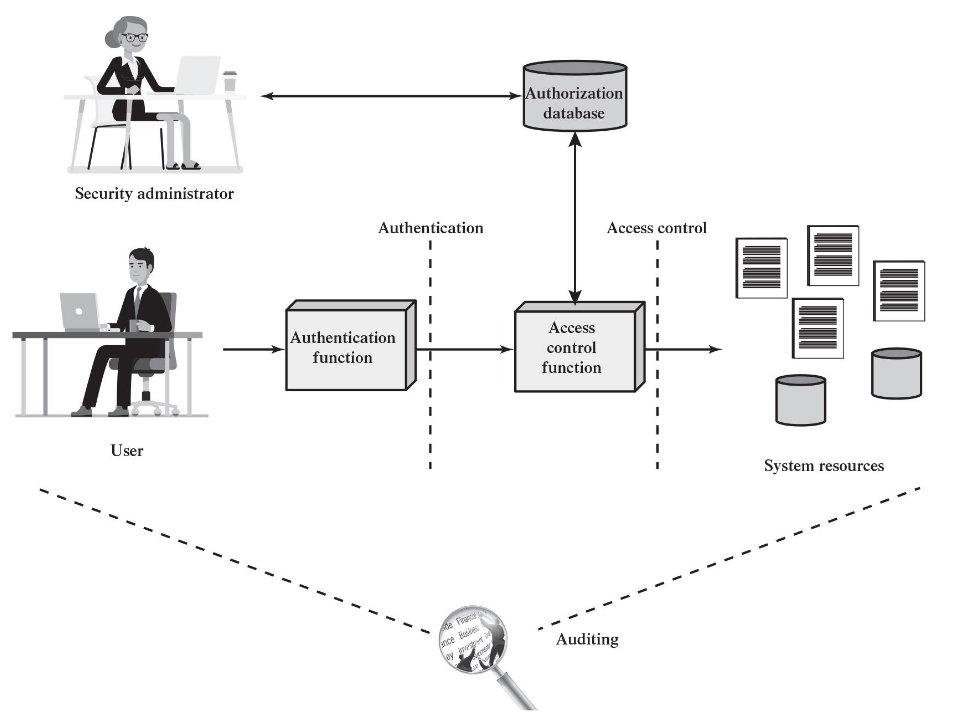
\includegraphics[width=0.4\textwidth]{img/Access Control Principles.png}
  \caption{Access Control Principles}
\end{figure}


\section{Relationship with Other Security Functions}
Access control interacts with several other security functions:

\begin{itemize}
    \item \textbf{Authentication}: Verifies user credentials before
      granting access.
    \item \textbf{Authorization}: Determines permissions based on
      policies and trust levels.
    \item \textbf{Audit}: Ensures compliance by reviewing system
      activities and identifying security breaches.
\end{itemize}

Administrators manage an authorization database, while authentication
functions verify users before granting access. Auditing provides an
independent review to maintain security compliance.

\section{Authentication and Audit}
Authentication ensures that a user or process is verified before accessing
system resources. Auditing plays a crucial role in maintaining security by
monitoring activities.

\subsection{Internal and External Audit}
IT enterprises conduct two types of audits:

\textbf{Internal Audit} is performed within the organization to identify risks
related to performance, security, and compliance. Internal auditors monitor
mitigation efforts to improve the organization’s security posture.

\textbf{External Audit} is conducted by independent professionals, often
Certified Public Accountants (CPAs), who assess an organization's security and
compliance. External audit reports are vital for stakeholders and clients.

\section{Access Control Mechanisms}
An access control mechanism regulates interactions between users and system
resources such as applications, operating systems, firewalls, routers, files,
and databases.

The process involves:

1. Authentication of the entity seeking access.
2. Authorization checks against an access control database.
3. Enforcement of access control policies.

Operating systems incorporate built-in access control functions, supplemented
by security add-ons and application-specific controls.

\section{Security Mechanisms and Policies}
Security mechanisms enforce policies through software and hardware functions.
The separation of policies from mechanisms allows flexibility in
implementation.

A security mechanism should:

- Independently define protection requirements.
- Compare different policies and enforcement mechanisms.
- Support multiple policies within the same system.

\subsection{Access Control Policies}
Access control policies define rules for regulating user access. They specify
what types of access are permitted, under what conditions, and by whom. These
policies can be formalized into authorization databases.

\section{Subjects, Objects, and Access Rights}
A well-defined access control system must identify:

- \textbf{Objects}: The resources requiring protection.
- \textbf{Subjects}: Entities requesting access.
- \textbf{Actions}: Operations performed on objects.

\textbf{Objects} include files, databases, messages, and programs. The number
and type of protected objects depend on system complexity and security
requirements.

\textbf{Subjects} represent active entities such as users, applications, and
processes. Subjects are accountable for their actions, with audit trails
recording relevant activities.

\textbf{Actions} refer to access operations such as Read, Write, Execute,
Delete, Create, and Search.

\section{Access Control Policy Models}
Access control policies are categorized into:

\textbf{Discretionary Access Control (DAC)}: Grants access based on user
identity and explicit authorization rules. Users can delegate their access
privileges to others.

\textbf{Mandatory Access Control (MAC)}: Enforces access restrictions based on
security labels and clearance levels. Users cannot override these restrictions.

\textbf{Role-Based Access Control (RBAC)}: Grants access based on
organizational roles rather than individual identities. Users inherit
permissions from their assigned roles.

\textbf{Attribute-Based Access Control (ABAC)}: Grants access based on
attributes of users, objects, and environmental conditions, offering a flexible
and dynamic approach.

\section{Implementation of Access Control}
Access control mechanisms are implemented using:

- \textbf{Access Control Lists (ACLs)}: Define permissions for each user-object
pair.
- \textbf{Capability Lists}: Assign access rights to subjects rather than
objects.
- \textbf{Authorization Tables}: Store access rules as a set of conditions.

\section{Advanced Access Control Concepts}
\subsection{Least Privilege and Separation of Privilege}
The principle of least privilege ensures that subjects are granted the minimum
access necessary to perform their tasks, reducing the risk of unauthorized
actions.

Separation of privilege divides access across multiple entities, requiring more
than one authorization to perform critical actions, thereby mitigating insider
threats.

\subsection{Role Hierarchies and Constraints in RBAC}
Role hierarchies allow roles to inherit permissions from superior roles.
Constraints define conditions such as:

- Mutually exclusive roles (a user can hold only one role in a set).
- Cardinality limits (restricting the number of users per role).
- Prerequisite roles (requiring users to hold a specific role before obtaining
another).

\subsection{ABAC and its Flexibility}
ABAC offers a powerful and flexible access control model by evaluating
attributes of subjects, objects, and environmental conditions. However, it
requires high computational effort, making it more complex than DAC and RBAC.

